\chapter{Conclusiones y Trabajos Futuros}
 \addcontentsline{toc}{chapter}{Conclusiones y Trabajos Futuros}

 \section{Conclusiones}

En estos momentos, una gran cantidad de datos es almacenada en bases de datos y almacenes de datos. Los datos crecen rápidamente porque la información se guarda usando periféricos de computadora, códigos de barras, sensores y sistemas biométricos. También una gran variedad de datos que se consideraban difíciles de manejar o que estaban aislados ahora tienen fines prácticos, estos datos son  grandes y complejos, con millones de registros y muchas variables. Además, diferentes agencias gubernamentales, instituciones educativas e industrias han acumulado estas grandes cantidades de datos. Como ejemplo, para el desarrollo de los objetivos de este proyecto de investigación la Facultad Nacional de Salud Publica  pone a disposición del Grupo de Investigación de Ingeniería y Tecnologías de las Organizaciones y de la Sociedad (ITOS) los Registros Individuales de Prestación de Servicios de Salud (RIPS) que se definen como el conjunto de datos mínimos y basicos  que el Sistema General de Salud Social requiere para sus procesos cuya denominación, estructura y características se ha unificado y estandarizado para todas las entidades a que hace referencia el artículo segundo de la resolución 3374 de 2000 (las instituciones prestadoras de servicios de salud (IPS), de los profesionales independientes, o de los grupos de práctica profesional, las entidades administradoras de planes de beneficios y los organismos de dirección, vigilancia y control del SGSSS.). Con estos datos se han llevado a cabo diferentes estudios y se sabe que son usados para diferentes indicadores de rendimiento (KPI), este trabajo de investigación brinda una forma de exportar estos indicadores y modelos, que no solo aplican para el dominio de la salud publica. Con el uso del estándar PMML, se logro exportar y reproducir sin necesidad de una plataforma robusta, los modelos que los científicos de datos desarrollan. Actualmente este estandar es poco usado y fue novedoso presentarlo como propuesta para el desarrollo de los modelos de características.\\

Por otra parte, al usar estudios sistemáticos  se redujo el sesgo en la investigación\cite{Petersen2015}, el resultado fue un estudio completo y replicable. Con los hallazgos realizados, se pudo seleccionar más fácilmente las técnicas de minería de datos que se aplicaron en la elaboración de los modelos de características. El SMS que se presento en la aplicación \textit{library} presentó un conjunto de documentos caracterizados y catalogados en una gran cantidad de dimensiones y características. 
En el diseño del prototipo se uso la base de datos (\textit{Iris}) muy conocida e interpretable por la comunidad, los resultados de los primeros modelos de caracteristicas provenientes del PMML de \textit{Iris} ayudaron considerablemente a abstraerse del formato e interiorizar los objetivos en el trabajo de investigación, puesto que el modelo que se generó con los datos de los RIPS, fue mas grande y desafiante. De acuerdo con esto, se conoce que las industrias son ricas en datos pero pobres en información\cite{Elovici2003}, y en el campo de la ILP los modelos de características son constituidos de cientos de características que aumentan la complejidad de la etapa de configuración en el proceso de la ILP\cite{Asadi2014}, la implementación de este desarrollo en \textit{Java} es un script que humildemente le dio la bienvenida a la creación de modelos de caracteristicas mediante técnicas estadísticas y computacionales que sean útiles en el ciclo de vida de ingeniería de líneas de producto. El desafio que se desprende es el uso de PMML para exportar los modelos que se realizan partiendo de esa gran cantidad de datos que se tiene en todos los diferentes dominios y contextos. Si se logra estandarizar nuestro proceso de descubrimiento de conocimiento en las bases de datos e incluir estos nuevos formatos es muy posible que las caracteristicas que impactan de forma positiva y negativa los intereses comerciales sean fácilmente identificables y que se minimicen los problemas de configuración cuando se piense en generar extensivamente productos personalizados.
\section{Trabajos futuros}
En el trabajo de investigación se detectó el estándar PMML como piedra angular de la codificación de los modelos en la minería de datos, desde esta perpectiva se pueden generar nuevos estudios sobre el uso de este formato o sobre la pertinencia del mismo o de XML para la representación y el transporte de la información. Los desarrollo en este trabajo fueron scripts aislados que no obedecen a ninguna arquitectura pero si a buenas practicas de desarrollo. Considerando lo anterior se propuso la Figura \ref{arquitecturadetalle} como representación de los futuros desarrollos obedeciendo un paradigma orientado a micro servicios.

 \begin{figure}[h]
	\centering
	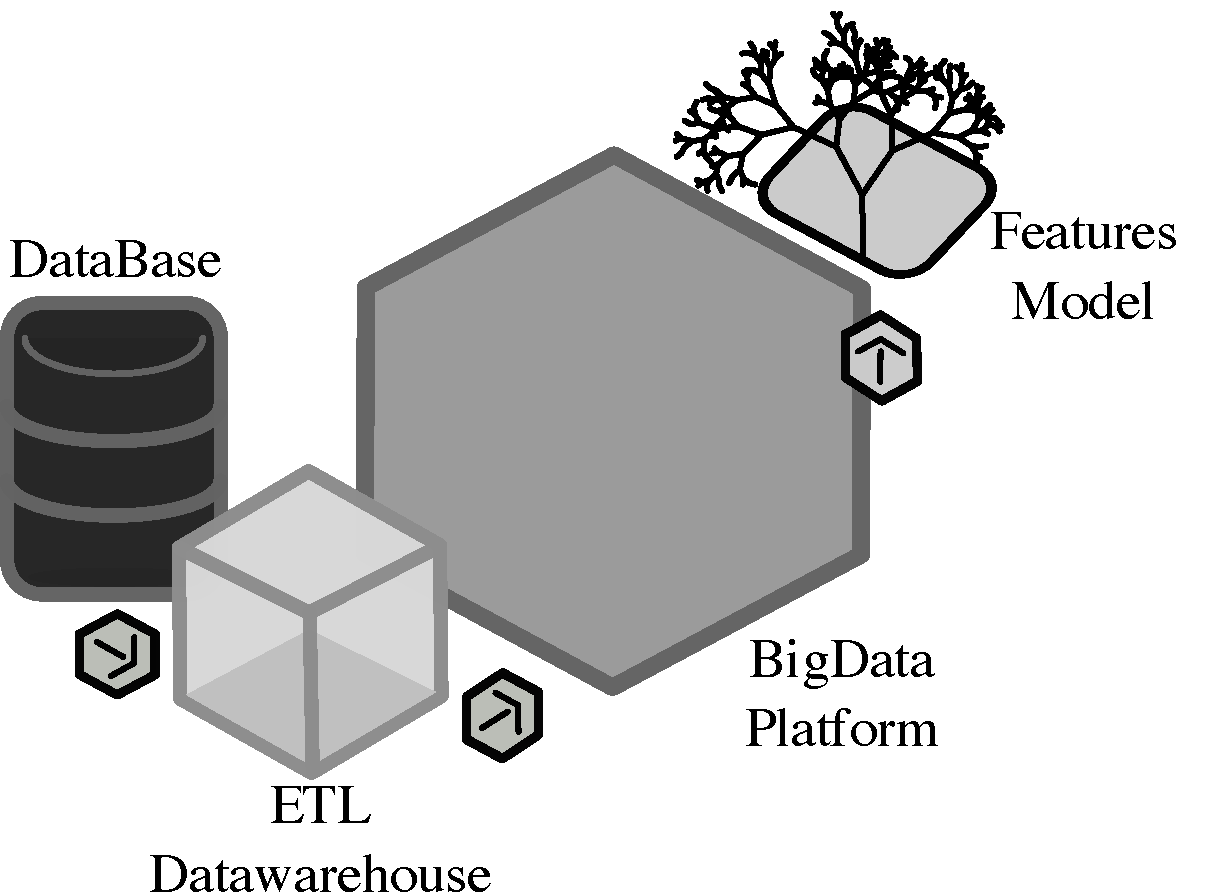
\includegraphics[scale=0.5]{arquitecturadetalle}
	\caption{Arquitectura a \textit{diez mil pies de altura} sobre el futuro de la integración del desarrollo con las nuevas tecnologías de \textit{BigData}.}
	\label{arquitecturadetalle}
\end{figure}

En la Figura \ref{arquitecturadetalle}, se simboliza el transito de la información con un hexágono, que parte de las bases de datos de sistemas legados por ejemplo, pasa por el proceso de extracción de conocimiento brindado por los algoritmos de extracción, transformación y cargar los datos, este proceso es actualmente un apéndice importante el las arquitecturas de \textit{BigData}. Luego, con los datos en un sistema de ficheros distribuido producto del uso de almacenes de datos o areas intermedias para el consumo de información, donde se puedan crear elegantes algoritmos concurrentes y hacer uso del paralelismo, se podría entonces mitigar los problemas de la alta dimensionalidad de los datos\cite{Izenman2006, Liang2015a}, sin embargo el desarrollo que se propuso(y los desarrollos industriales modernos) debería de adaptarse primero a una arquitectura SOA y desarrollar un componente de integración o adaptar un patron empresarial existente, en el que se ofresca un servicio que el futuro se pueda desplegar en un arquitectura de micro servicios, siendo consecuentes con esta idea se desarrollo usando un administrador de código fuente y el \href{https://maven.apache.org/guides/introduction/introduction-to-the-pom.html}{\textit{POM}} como artefacto fundamental para el trabajo con \textit{maven} y la filosofía de entrega continua e integración continua.